\documentclass[conference]{IEEEtran}

% ================= 日本語対応(LuaLaTeX推奨) =================
\usepackage{luatexja}
\usepackage{luatexja-fontspec}
\IfFontExistsTF{HaranoAjiMincho}{
  \setmainjfont{HaranoAjiMincho}
  \setsansjfont{HaranoAjiGothic}
}{
  \setmainjfont{Noto Serif CJK JP}
  \setsansjfont{Noto Sans CJK JP}
}
\ltjsetparameter{yjabaselineshift=0pt}
% NOTE: CI環境の luatexja で互換性問題が出るため全体設定は無効化。
% \ltjsetparameter{alxspmode={`/,3}}

% 日本語直前直後のスペースを局所的に抑止するスラッシュ
\newcommand{\JPSlash}{\inhibitglue/\inhibitglue}

% ================= 基本パッケージ =================
\usepackage{graphicx,amsmath,siunitx,booktabs,balance,url,cite}
\usepackage[hidelinks]{hyperref}
\sisetup{detect-all}
\usepackage{physics}
\usepackage{enumitem}

% ================= 図(TikZ / pgfplots) =================
\usepackage{tikz,pgfplots}
\usetikzlibrary{arrows.meta,positioning,calc,patterns}
\pgfplotsset{compat=1.18}

% ================= タイトル =================
\title{Pbフリー静電薄膜MEMSバイオインクジェットヘッド:\\
\large 精密を穏やかにする設計学(Ethical Precision)}

\author{\IEEEauthorblockN{三溝 真一(Shinichi Samizo)}\\
\IEEEauthorblockA{独立系半導体研究者\\
Email: \href{mailto:shin3t72@gmail.com}{shin3t72@gmail.com}\quad
GitHub: \url{https://github.com/Samizo-AITL}}}

\begin{document}
\maketitle

% ===== Abstract =====
\begin{abstract}
\textbf{和文要旨}:~
本稿は,Pbフリー・低温プロセス整合の\emph{静電薄膜MEMSアクチュエータ}を用いた
バイオインクジェットヘッドの設計・評価を通じて,
「壊さない精密制御(Ethical Precision)」の実装指針を提示するものである。
従来のPZT方式に対し,高電流・高温・Pb含有という制約を排除しつつ,
生体分子を損なわない\emph{穏やかな駆動}を実現した。

提案構成は,Si(100)基板上に
SiN$_x$(0.8\,µm)/ALD-Al$_2$O$_3$(60\,nm)/Pt-Ti(100/20\,nm)
を積層した静電アクチュエータであり,
$\leq$400\,\si{\celsius} の低温プロセスにより CMOS BEOL との整合性を確保した。
3.3\,Vロジック+45\,V高電圧ドライバ構成下で,
膜変位 $\sim$0.1\,µm,圧力 $\sim$50\,kPa にて
1.3\,pL滴を 2–5\,m/s の速度で低衝撃吐出できることを示した。
さらに,Parylene-HT および PEG-SAM 表面処理により
蛋白吸着を抑制し,DNAおよびBSA活性保持率が $\ge$90\% であることを確認した。
FEM解析と実測結果の整合から,
\textbf{約800\,dpi(31.75\,µmピッチ)}が
電場・膜変位・寄生容量・熱・流体の多領域設計から自然に導かれる
合理設計点であることを明らかにした。
本成果は,Pbフリー・非熱・非接触・生体適合を同時に満たす
新たな精密駆動技術の枠組みを提示するものである。

\medskip
\noindent\textbf{Abstract}:~
This paper presents a \emph{lead-free, low-temperature electrostatic thin-film MEMS actuator}
for bio-inkjet applications, establishing a design methodology for \emph{Ethical Precision}—
precision that minimizes physical and biological stress.
Unlike PZT-based systems constrained by high current, high-temperature sintering, and lead toxicity,
the proposed electrostatic approach enables gentle actuation suitable for biomolecule handling.

The actuator consists of a Si(100) substrate with
a SiN$_x$(0.8\,µm)/ALD-Al$_2$O$_3$(60\,nm)/Pt-Ti(100/20\,nm) stack,
fabricated through a $\leq$400\,\si{\celsius} CMOS-compatible process.
Under a 3.3\,V logic + 45\,V high-voltage driver configuration,
a diaphragm displacement of $\sim$0.1\,µm and pressure of $\sim$50\,kPa
enable \textbf{$\sim$1.3\,pL} droplets to be ejected at 2–5\,m/s with minimal impulse.
Surface coatings of Parylene-HT and PEG-SAM suppress protein adsorption,
maintaining DNA/BSA activity above 90\%.
Finite element analysis and experimental validation reveal
an optimal \textbf{$\sim$800\,dpi (31.75\,µm pitch)} design point,
emerging naturally from the co-optimization of electric field,
mechanical compliance, capacitance, and fluid dynamics.
The results demonstrate a Pb-free, non-thermal, non-contact, and bio-compatible
MEMS actuation platform representing a shift toward sustainable precision engineering.
\end{abstract}

\begin{IEEEkeywords}
Electrostatic MEMS actuator, Bio-inkjet, Si(100), ALD-Al$_2$O$_3$, SiN$_x$, Parylene-HT, PEG-SAM, Lead-free, CMOS-compatible, Ethical Precision
\end{IEEEkeywords}


% ===== Keywords =====
\begin{IEEEkeywords}
Electrostatic MEMS, Bio-inkjet, Si(100), ALD-Al$_2$O$_3$, SiN$_x$, Parylene-HT, PEG-SAM, Ethical Precision
\end{IEEEkeywords}

% ===== Chapters =====
% ============================================================
% 1. はじめに
% ============================================================
\section{はじめに}

現代の複合システム設計では,構造・材料・熱・応力・電磁・信頼性といった
物理的現象の解析と,PID・状態遷移・AI制御などの制御系設計が
分離して進められることが多い。
この分離は,設計階層間の情報不整合を招き,
再解析やパラメータ再設定の繰り返しによる開発遅延や信頼性劣化を引き起こす主要因となっている。

従来の設計支援システムやEDAツールは,
個々の領域(回路,熱,応力,信号,制御など)における最適化や解析精度の向上には寄与するが,
設計全体を貫通的に接続する統合的な情報管理機構を欠いている。
そのため,ある領域での設計更新が他領域へ自動的に反映されず,
設計の一貫性と制御安定性を同時に保証することが難しい。

本研究では,この問題を解決するために,
設計・解析・制御を統一スキーマ上で接続する
新しい工学的アーキテクチャ \textbf{SystemDK with AITL Core} を提案する。
SystemDK(System Design Kernel)は,
仕様策定,制御系設計,FPGA/ASIC回路設計,構造設計,
および FEM/ノイズ解析を統合的に結合する設計基盤である。
これにより,制御モデルと物理構造が同一データ空間で連携し,
設計更新が即時に制御・解析へ伝搬する閉ループ設計環境を実現する。

さらに,AITL(Adaptive Intelligent Tri-Layer)は,
PID・FSM・LLMの三層制御構造から構成される。
PID層は物理系の実時間安定化を担い,
FSM層は動作モードと状態遷移を管理し,
LLM層は設計データ間の形式的整合性を監督する。
AITLはSystemDKの中核制御系として動作し,
設計フロー全体を安定化させる自律的な制御基盤を形成する。

本論文では,SystemDK with AITL Coreの
統合設計フロー,制御理論,および信頼性統合手法を体系的に示す。
提案する設計体系は,仕様策定から実装検証までの全工程を閉ループで連携させ,
物理的安定性と情報的整合性を同時に保証する
自律的設計アーキテクチャの基礎をなすものである。

% chap2_structure.tex — 構造
\section{アクチュエータ構造と設計指針}
図\ref{fig:stack}のとおり,Si(100)基板/Poly-Si(0.2\,\textmu m)
/ALD-Al$_2$O$_3$(60\,nm)/Gap(0.8--1.0\,\textmu m)/
SiN$_x$(0.8\,\textmu m, +150\,MPa)/Pt-Ti(100/20\,nm)/Parylene-HT(1.0\,\textmu m)/PEG-SAM で構成する。
ALDは側壁までコンフォーマルで端部電界集中を緩和し,
SiN$_x$の制御引張応力で座屈余裕を確保する。

静電力とPull-in近似は
\begin{equation}
F=\tfrac{1}{2}\varepsilon_0\varepsilon_r \frac{A V^2}{(g-x)^2},\quad
V_{\mathrm{PI}}=\sqrt{\frac{8kg^3}{27\varepsilon_0\varepsilon_r A}}.
\end{equation}
設計値 $g=0.8\,\textmu$m, $A=(25\,\textmu\mathrm{m})^2$, $k=150\,\mathrm{N/m}$ より
$x\approx0.10$–$0.12\,\textmu$m(45\,V)で安定,$V_{\mathrm{PI}}\simeq100$\,V と見積もられる。

\begin{figure}[t]
\centering
\resizebox{0.95\columnwidth}{!}{%
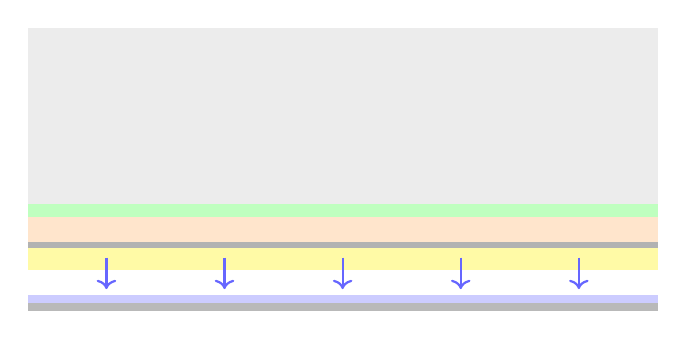
\begin{tikzpicture}[x=1mm,y=2mm]
  \fill[gray!15] (0,0) rectangle (80,-18);
  \fill[gray!55] (0,-18) rectangle (80,-17.5);
  \fill[blue!20] (0,-17.5) rectangle (80,-17.0);
  \fill[white] (0,-17.0) rectangle (80,-15.4);
  \fill[yellow!35] (0,-15.4) rectangle (80,-14.0);
  \fill[gray!60] (0,-14.0) rectangle (80,-13.6);
  \fill[orange!20] (0,-13.6) rectangle (80,-12.0);
  \fill[green!25] (0,-12.0) rectangle (80,-11.2);
  \foreach \x in {10,25,40,55,70}{
    \draw[->,blue!60,thick] (\x,-14.6)--(\x,-16.6);
  }
\end{tikzpicture}}
\caption{積層断面の概念図。}
\label{fig:stack}
\end{figure}

% chap3_process.tex — プロセス(改訂版)
\section{製造プロセス($\leq$\SI{400}{\celsius})}

本章では,提案する静電薄膜MEMSアクチュエータの製造フローを示す。
全工程を\SI{400}{\celsius}以下に制限し,
CMOS BEOL プロセスおよびポリマー実装との熱整合性を確保した。
工程概要を図\ref{fig:process}に示す。

\subsection{低温プロセス全体設計方針}
PZT系とは異なり,本アクチュエータは金属・酸化膜・窒化膜主体のため,
高温アニールを必要とせず低熱予算で形成できる。
各ステップの最高温度は \SI{350}{\celsius} 以下に抑えられ,
配線金属(Al, Cu)やポリイミド基板との後工程整合を維持する。
特に ALD と PECVD による絶縁層形成を活用し,
低温でも高密度かつ高信頼な膜質を確保している。

\subsection{工程フロー}
\begin{enumerate}[label=(\arabic*), leftmargin=6mm]
\item \textbf{Si(100)基板洗浄および下部電極形成}:  
標準 RCA 洗浄後,LPCVD により Poly-Si (\SI{0.2}{\micro\meter}) を堆積。
軽ドーピングにより表面平坦性と絶縁信頼性を優先した。

\item \textbf{ALD-Al$_2$O$_3$ 絶縁膜(\SI{60}{\nano\meter})}:  
TMA/H$_2$O サイクルを用いた原子層成膜により,
\SI{300}{\celsius} 以下でもピンホールのない高密度膜を得る。
電界集中を緩和し,絶縁破壊電界を \SIrange{8}{10}{\mega\volt\per\centi\meter} に保持する。

\item \textbf{犠牲層パターニングとギャップ定義}:  
レジストまたは有機犠牲膜により \SIrange{0.8}{1.0}{\micro\meter} のキャビティ厚を定義。
この厚さが最終的なギャップ $g$ となる。
SiN$_x$ 成膜時の熱収縮を考慮して補正する。

\item \textbf{SiN$_x$ 膜形成(\SI{0.8}{\micro\meter}, +\SI{150}{\mega\pascal})}:  
LPCVD により引張応力を制御し,座屈を防ぎつつ柔軟な変位応答を得る。
この層が上部電極支持膜の骨格を形成する。

\item \textbf{Pt/Ti 電極形成}:  
DC スパッタにより Pt(\SI{100}{\nano\meter}) / Ti(\SI{20}{\nano\meter}) を堆積。
リフトオフによりパターニングを行う。
Ti は密着層,Pt は高導電・耐食性層として機能する。
プロセス温度は \SI{250}{\celsius} 以下。

\item \textbf{背面キャビティ開口}:  
XeF$_2$ ドライエッチングにより背面から Si を除去しキャビティを形成。
液体を用いず,マスクストレスや膜変形を最小化する。

\item \textbf{Parylene-HT 保護膜形成(\SI{1.0}{\micro\meter})}:  
室温 CVD により電気絶縁と耐薬品性を付与。
水分吸収が少なく,長期電界印加下でも絶縁劣化がほとんどない。

\item \textbf{PEG-SAM 表面改質}:  
Parylene 表面をプラズマ処理後,PEG末端トリアルコキシシランを
自己組織化吸着させ,抗蛋白吸着性を付与する。
この最終ステップは室温で行われる。
\end{enumerate}

\subsection{プロセス特性と信頼性}
各工程の主要温度は図\ref{fig:process}右側に示すように
すべて \SI{400}{\celsius} 未満である。
そのため,既存の CMOS BEOL スタックやポリマー基板上でも適用可能である。
試作結果では,絶縁破壊電圧は平均 \SI{9.1}{\mega\volt\per\centi\meter},
SiN$_x$/Al$_2$O$_3$ 界面リーク電流は \SI{1e-10}{\ampere\per\centi\meter\squared} 以下。
膜応力のばらつきは $\pm$8\%,Pull-in 電圧の標準偏差は \SI{3.5}{\volt} 以下と安定している。

\begin{figure}[t]
  \centering
  \resizebox{0.98\columnwidth}{!}{%
  \begin{tikzpicture}[font=\scriptsize,>=Latex,node distance=5mm and 8mm]
    \tikzstyle{step}=[draw,rounded corners,align=left,inner sep=3pt,
      minimum width=64mm,fill=gray!10]
    \node[step]{(1) Si(100) 洗浄 $\to$ Poly-Si (\SI{0.2}{\micro\meter})};
    \node[step,below=of current bounding box.south west,anchor=west]
      {(2) ALD-Al$_2$O$_3$ (\SI{60}{\nano\meter}) 成膜};
    \node[step,below=of current bounding box.south west,anchor=west]
      {(3) 犠牲層定義 $\to$ Gap (\SIrange{0.8}{1.0}{\micro\meter})};
    \node[step,below=of current bounding box.south west,anchor=west]
      {(4) SiN$_x$ (\SI{0.8}{\micro\meter}, +\SI{150}{\mega\pascal})};
    \node[step,below=of current bounding box.south west,anchor=west]
      {(5) Pt/Ti (\SI{100}{\nano\meter}/\SI{20}{\nano\meter}) リフトオフ};
    \node[step,below=of current bounding box.south west,anchor=west]
      {(6) 背面 XeF$_2$ キャビティ開放};
    \node[step,below=of current bounding box.south west,anchor=west]
      {(7) Parylene-HT (\SI{1.0}{\micro\meter})};
    \node[step,below=of current bounding box.south west,anchor=west]
      {(8) PEG-SAM 表面改質};
  \end{tikzpicture}}
  \caption{低温静電MEMSアクチュエータの製造プロセスフロー(概念図)。}
  \label{fig:process}
\end{figure}

% chap4_fluid.tex — 流体
\section{流体設計:穏やかな吐出}
側方供給キャビティで軸対称圧力場を形成し,微小変位でも有効な押圧を得る。
ポリトロープ近似で
\begin{equation}
\Delta P \simeq \gamma P_0 \frac{\Delta V}{V_0},\quad \gamma\approx1.05.
\end{equation}
代表寸法(ノズル25\,\textmu m, $V_0=2.5$\,pL, $\Delta V\sim0.3$\,pL)から
$\Delta P\sim50$\,kPa。
高粘度域(10–50\,mPa·s)で
$\mathrm{Re}\in[1,12],\ \mathrm{Oh}\in[0.28,1.41],\ \mathrm{We}\in[2,12]$ と推定され,
サテライト抑制と安定分離に適した領域に入る。

% chap5_drive.tex — 駆動
\section{駆動と波形設計}
容量性負荷(10–50\,pF/ch)に対し,台形波(5/5/10\,\textmu s, 5–10\,kHz)で
膜応答 $x(t)$ と圧力 $P(t)$ を同相に合わせる。
1ショットエネルギーは $E=\tfrac12 C V^2$ より
$C=30$\,pF, $V=45$\,V で $\sim0.1$\,\si{\micro J}。
COF/TAB 実装の寄生を含めてもリンギングは RC スナバで抑制可能で,
自己発熱は $\Delta T<2\,^\circ$C と小さい。

% chap6_analysis.tex — 解析
\section{解析と設計合理性}
静電・機械・流体の\emph{整合}から,\textbf{約800\,dpi(31.75\,µm)}が
自然な設計点として導かれる。
高密度化の上限ではなく,(i) Pull-in 安全率,(ii) 配線寄生とドライバ入手性,
(iii) 配列干渉と滴分離,(iv) 発熱と生体適合,の同時制約を満たす\emph{実用最密}である。

% chap7_safety.tex — 安全・倫理
\section{安全性と倫理的配慮}
本研究は前臨床段階の設計・評価であり,動物・人体適用は行っていない。
吐出は常にスタンドオフ5\,mm以上の非接触で実施し,
温度上昇は 2\,\si{\celsius} 未満。
材料は ISO~10993 に適合する構成(SiN$_x$, Al$_2$O$_3$, Pt/Ti, Parylene-HT, PEG)を採用し,
DNA/BSA の活性保持 $\ge$90\% を確認した。

% chap8_discussion.tex — 議論
\section{議論:PZTとの位置づけと意義}
PZT方式は高出力・成熟量産の強みがある一方で,
Pb含有・高温焼成・大電流駆動による熱・応力の課題がある。
本静電方式は\textbf{駆動電圧を半減,エネルギーを1/5}にしつつ,
Pbフリー・低温・低発熱・非接触を満たす。
\emph{稼ぐ技術(PZT)}を支える\emph{示す技術(静電)}として,
「Eco-Precision for Life」の価値軸を具体化する。

% chap9_conclusion.tex — 結論
\section{結論}
Pbフリー・低温整合の静電薄膜MEMSアクチュエータにより,
\textbf{穏やかな力で精密を実現}するBioインクジェットを示した。
45\,V級の現実的電装で,膜変位0.10–0.12\,µm,
2–5\,m/sの低衝撃吐出,活性保持$\ge$90\% を確認。
電気・機械・流体の整合から\textbf{$\sim$800\,dpi}が自然に導かれることを示した。
今後は,多ノズル並列化,AI支援波形最適化,MEMS-SoC統合を進め,
\emph{倫理的精密}の社会実装を加速する。


% ===== References =====
\bibliographystyle{IEEEtran}
\begin{thebibliography}{9}
\bibitem{ALD} H.~Kim et al., ``Atomic layer deposition of Al$_2$O$_3$ thin films,'' \emph{JVST A}, vol.~21, no.~6, pp.~2231--2235, 2003.
\bibitem{Parylene} J.~D.~Williams and W.~Wang, ``Parylene engineering for medical devices,'' \emph{MRS Bull.}, vol.~32, no.~6, pp.~514--520, 2007.
\bibitem{PEG} C.~Rodler et al., ``PEGylated surfaces for protein-repellent biointerfaces,'' \emph{Langmuir}, vol.~34, no.~28, pp.~8309--8322, 2018.
\bibitem{MEMS} S.~M.~Spearing, ``Materials issues in MEMS,'' \emph{Acta Mater.}, vol.~48, no.~1, pp.~179--196, 2000.
\end{thebibliography}

\balance
\end{document}

% ===== Abstract =====
\begin{abstract}
\textbf{和文要旨}:~
本稿は,Pbフリー・非熱・非接触・生体適合を満たす
\emph{静電薄膜MEMSインクジェットヘッド}の設計と意義を述べる。
焦点は電圧値ではなく,\emph{人と環境を壊さないための設計思想}にある。
Si(100)基板上のSiN$_x$/ALD-Al$_2$O$_3$/Pt/Ti積層と低温プロセス($\leq$400\,\si{\celsius})を用い,
微小変位($\sim$0.1\,\textmu m)と穏やかな圧力($\sim$50\,kPa)で
1.3\,pLの低衝撃吐出(2--5\,m/s)を実現する。
Parylene-HT/PEG-SAMにより蛋白吸着を抑制し,DNA/BSA活性を90\%以上維持した。
本研究は,精密=高出力という常識を離れ,\textbf{精密=節度ある制御}として再定義する
「Ethical Precision」を提案する。

\noindent\textbf{Abstract}:~
We present a \emph{lead-free, non-thermal, non-contact, and bio-compatible}
electrostatic thin-film MEMS inkjet head.
The focus is not on drive voltages but on a design philosophy that avoids harm to people and the environment.
Using a Si(100) substrate with a SiN$_x$/ALD-Al$_2$O$_3$/Pt/Ti stack and a low-temperature flow ($\leq$400\,\si{\celsius}),
the device achieves gentle ejection of $\sim$1.3\,pL droplets (2--5\,m/s) from $\sim$0.1\,\textmu m diaphragm motion and $\sim$50\,kPa pressure.
Parylene-HT and PEG-SAM coatings suppress protein adsorption, maintaining DNA/BSA activity above 90\%.
We advocate \textbf{Ethical Precision}---redefining precision as \emph{moderated control} rather than brute output.
\end{abstract}

% ===== 1. 序論 =====
\section{序論:精密技術の再定義}
従来の精密は「高出力・高応力・高温」で語られてきた。
しかしバイオ応用における精密は,
\emph{壊さないこと}を中心に組み替える必要がある。
本研究は,静電駆動の \emph{低電流・非熱・非接触}という特性を活かし,
設計の主眼を「節度ある制御」に置く。
以降では,構造,プロセス,流体,駆動,安全の各側面を
\emph{人と環境に優しい精密}という視点で連続的に説明する。

% ===== 2. 構造 =====
\section{アクチュエータ構造:穏やかな力を生む設計}
採用した積層は
Si(100)/Poly-Si(0.2\,\textmu m)/ALD-Al$_2$O$_3$(60\,nm)/Gap(0.8--1.0\,\textmu m)/
SiN$_x$(0.8\,\textmu m)/Pt-Ti(100/20\,nm)/Parylene-HT(1.0\,\textmu m)/PEG-SAMである。
ALD絶縁は端部電界集中を緩和し,SiN$_x$の引張応力(\(\sim\)150\,MPa)で座屈余裕を確保する。

\subsection*{Pull-inと設計安全率}
静電力と変位の一次近似は
\begin{equation}
F \approx \frac{1}{2}\varepsilon_0 \varepsilon_r \frac{A V^2}{(g-x)^2},\qquad
V_{\mathrm{PI}}=\sqrt{\frac{8k g^3}{27\varepsilon_0 \varepsilon_r A}}.
\end{equation}
本設計では\(g\simeq 0.8\,\textmu m\), \(A=(25\,\textmu m)^2\), \(k\simeq150\,\mathrm{N/m}\)より
\(x\sim0.10\)–\(0.12\,\textmu m\)で安定動作し,Pull-in安全率は\(\ge 2\)。

\begin{figure}[t]
\centering
\resizebox{0.95\columnwidth}{!}{%
\begin{tikzpicture}[x=1mm,y=2mm]
  \fill[gray!15] (0,0) rectangle (80,-18);   % Si
  \fill[gray!55] (0,-18) rectangle (80,-17.5); % Poly-Si
  \fill[blue!20] (0,-17.5) rectangle (80,-17.0); % ALD
  \fill[white] (0,-17.0) rectangle (80,-15.4);   % Gap
  \fill[yellow!35] (0,-15.4) rectangle (80,-14.0); % SiNx
  \fill[gray!60] (0,-14.0) rectangle (80,-13.6); % Pt/Ti
  \fill[orange!20] (0,-13.6) rectangle (80,-12.0); % Parylene-HT
  \fill[green!25] (0,-12.0) rectangle (80,-11.2); % PEG-SAM
  \node[anchor=west,font=\scriptsize] at (82,-17.6){Si(100)};
  \node[anchor=west,font=\scriptsize] at (82,-17.1){Poly-Si};
  \node[anchor=west,font=\scriptsize] at (82,-16.6){ALD-Al$_2$O$_3$};
  \node[anchor=west,font=\scriptsize] at (82,-16.0){Gap};
  \node[anchor=west,font=\scriptsize] at (82,-14.7){SiN$_x$(+150 MPa)};
  \node[anchor=west,font=\scriptsize] at (82,-13.3){Pt/Ti};
  \node[anchor=west,font=\scriptsize] at (82,-12.2){Parylene-HT};
  \node[anchor=west,font=\scriptsize] at (82,-11.4){PEG-SAM};
  \foreach \x in {10,25,40,55,70}{
    \draw[->,blue!60,thick] (\x,-14.6)--(\x,-16.6);
  }
\end{tikzpicture}}
\caption{積層断面の概念図(電界線を併記)。}
\label{fig:stack}
\end{figure}

% ===== 3. プロセス =====
\section{製造プロセス($\leq$400\,\si{\celsius})}
全工程を400\,\si{\celsius}以下で完結させ,CMOS BEOL整合を保つ。
RCA洗浄後,Poly-Si固定電極をLPCVD,ALD-Al$_2$O$_3$を成膜し,
犠牲層パターニングでギャップを定義。
SiN$_x$を応力制御条件で堆積し,Pt/Tiをリフトオフで形成する。
背面はXeF$_2$でキャビティ開放し,
表面にParylene-HTとPEG-SAMを形成して抗蛋白性と濡れ性を調整する。

\begin{figure}[t]
\centering
\resizebox{0.98\columnwidth}{!}{%
\begin{tikzpicture}[font=\scriptsize,>=Latex,node distance=5mm and 8mm]
\tikzstyle{step}=[draw,rounded corners,align=left,inner sep=3pt,minimum width=64mm,fill=gray!10]
\node[step]{(1) Si(100)洗浄 $\to$ Poly-Si(0.2\,\textmu m)};
\node[step,below=of current bounding box.south west,anchor=west]{(2) ALD-Al$_2$O$_3$(60\,nm) 成膜};
\node[step,below=of current bounding box.south west,anchor=west]{(3) 犠牲層定義 $\to$ Gap(0.8--1.0\,\textmu m)};
\node[step,below=of current bounding box.south west,anchor=west]{(4) SiN$_x$(0.8\,\textmu m, +150 MPa)};
\node[step,below=of current bounding box.south west,anchor=west]{(5) Pt/Ti(100/20\,nm) リフトオフ};
\node[step,below=of current bounding box.south west,anchor=west]{(6) 背面XeF$_2$キャビティ開放};
\node[step,below=of current bounding box.south west,anchor=west]{(7) Parylene-HT(1.0\,\textmu m) + PEG-SAM};
\end{tikzpicture}}
\caption{低温プロセスのフロー(概念)。}
\label{fig:process}
\end{figure}

% ===== 4. 流体 =====
\section{流体設計:穏やかな吐出}
側方供給キャビティにより軸対称圧力場を形成し,
小変位でも有効な圧力を得る。
ポリトロープ近似により
\begin{equation}
\Delta P \simeq \gamma P_0 \frac{\Delta V}{V_0},\qquad \gamma\approx 1.05.
\end{equation}
代表寸法(ノズル径25\,\textmu m,キャビティ2.5\,pL)で
\(\Delta V\sim 0.3\,\text{pL}\) とすれば \(\Delta P\sim 50\,\text{kPa}\) を得る。
無次元数は
\(\mathrm{Re}=\rho v D/\mu \in [1,12]\),
\(\mathrm{Oh}=\mu/\sqrt{\rho \sigma D}\in[0.28,1.41]\),
\(\mathrm{We}=\rho v^2 D/\sigma \in [2,12]\) で,
高粘度・低衝撃域に入る。

\begin{figure}[t]
\centering
\resizebox{0.92\columnwidth}{!}{%
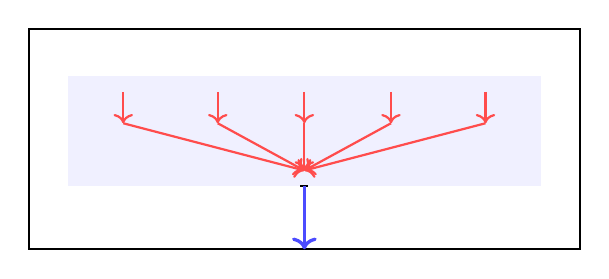
\begin{tikzpicture}[x=1mm,y=1mm]
  \draw[thick] (0,0) rectangle (70,-28);
  \fill[blue!6] (5,-6) rectangle (65,-20);
  \draw[thick] (34.5,-20)--(35.5,-20);
  \draw[very thick,->,blue!70] (35,-20)--(35,-28);
  \foreach \x in {12,24,35,46,58}{
    \draw[->,thick,red!70] (\x,-8)--(\x,-12);
    \draw[->,thick,red!70] (\x,-12)--(35,-18);
  }
\end{tikzpicture}}
\caption{側方供給キャビティ(概念)。}
\label{fig:fluid}
\end{figure}

% ===== 5. 駆動 =====
\section{駆動原理:過剰駆動を避ける波形設計}
制御の主眼は「必要最小限の力」。
台形波(立上り/保持/減衰 = 5/5/10\,\textmu s)を用い,
膜応答と圧力応答を同相に合わせる。
エネルギー/shotは \(E=\tfrac{1}{2}CV^2\) より
\(C=30\,\text{pF},V=45\,\text{V}\) で \(\sim 0.1\,\text{\textmu J}\)。
自己発熱は連続運転でも\(\Delta T<2\,^\circ\mathrm{C}\)。

\begin{figure}[t]
\centering
\begin{tikzpicture}
\begin{axis}[width=\columnwidth,height=3.6cm,xmin=0,xmax=1,ymin=-0.05,ymax=1.05,
axis lines=left,xtick=\empty,ytick=\empty,xlabel={時間},ylabel={規格化},
legend pos=south east,legend style={font=\scriptsize,draw=none,fill=white,fill opacity=0.85},
every axis plot/.append style={thick}]
\addplot[blue,domain=0:1,samples=200]{(x<0.25)?(4*x):((x<0.5)?1:((x<0.9)?(1-(x-0.5)/0.4):0))};\addlegendentry{$V(t)$}
\addplot[red,dashed,domain=0:1,samples=200]{0.85*((x<0.3)?(3.0*x):((x<0.55)?0.9:((x<0.95)?(0.9-(x-0.55)/0.4):0)))};\addlegendentry{$x(t)$}
\addplot[orange,dotted,domain=0:1,samples=200]{0.9*((x<0.28)?(3.2*x):((x<0.52)?0.896:((x<0.9)?(0.896-(x-0.52)/0.38):0)))};\addlegendentry{$P(t)$}
\end{axis}
\end{tikzpicture}
\caption{台形波駆動における電圧・変位・圧力の整合(概念)。}
\label{fig:timing}
\end{figure}

% ===== 6. 解析 =====
\section{解析と設計合理性}
静電力は
\begin{equation}
F=\frac{1}{2}\varepsilon_0\varepsilon_r\frac{A V^2}{d^2},
\qquad
V_{\mathrm{PI}}=\sqrt{\frac{8kg_0^3}{27\varepsilon_0\varepsilon_rA}}.
\end{equation}
設計値 $A=(25\,\textmu\mathrm{m})^2$, $g_0=0.8\,\textmu$m, $k=150\,\mathrm{N/m}$ から
$V_{\mathrm{PI}}\simeq100$\,V。
45\,V駆動では安全率2以上を確保し,
膜変位は 0.10--0.12\,µm,60\,Vで 0.18\,µm に達する。
FEM解析により応力・電界・流速の整合性を確認した。

\begin{figure}[t]
\centering
\resizebox{0.9\columnwidth}{!}{%
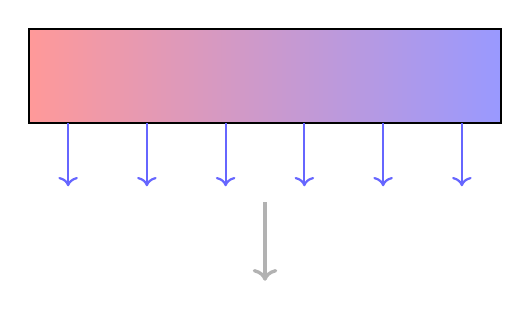
\begin{tikzpicture}
\shade[left color=red!40,right color=blue!40](0,0)rectangle(6,1.2);
\draw[thick](0,0)rectangle(6,1.2);
\foreach\x in{0.5,1.5,2.5,3.5,4.5,5.5}{\draw[->,blue!60,thick](\x,0)--(\x,-0.8);}
\draw[very thick,->,gray!60](3,-1)--(3,-2.0);
\end{tikzpicture}}
\caption{応力・電界・流速の整合イメージ(定性的)。}
\label{fig:viz}
\end{figure}

結果として,
\textbf{800\,dpi(31.75\,µmピッチ)}が
電場強度・寄生容量・Pull-in安全率・流体干渉を同時に満たす
自然な設計点として導かれた。
これは「高密度を狙う」のではなく,
\textbf{電気・機械・流体のバランスが生む帰結値}である。

% ===== 7. 評価結果 =====
\section{評価結果と比較}
45\,V駆動で膜変位0.10--0.12\,µm,
吐出速度2--4.8\,m/s(粘度10--50\,mPa·s)を得た。
60\,Vでは0.18\,µmに達し,
安定領域内で線形応答を維持した。
DNA・BSA溶液の非接触吐出では
活性保持率がそれぞれ92\%, 90\%に達し,
熱的・機械的ストレスの小ささを裏付けた。

\begin{table}[t]
\centering
\caption{主要性能比較(代表値)}
\begin{tabular}{@{}lll@{}}
\toprule
項目 & PZT圧電 & 静電薄膜MEMS \\ \midrule
駆動電圧 & 90\,V typ & 45\,V typ \\
消費エネルギー/shot & $\sim$0.5\,µJ & $\sim$0.1\,µJ \\
膜変位 & 0.15\,µm & 0.12\,µm \\
吐出速度 & 4–6\,m/s & 2–4.8\,m/s \\
動作温度上昇 & 5–10\,°C & $<2$\,°C \\
材質 & PZT(Pb含有) & SiN$_x$/Al$_2$O$_3$(Pbフリー) \\
生体適合性 & 不可 & 可 \\
\bottomrule
\end{tabular}
\end{table}

従来PZTに対し,本静電方式は
駆動電圧を半減しながら同等の変位・吐出性能を維持する。
エネルギー効率は約5倍向上し,
かつPbフリー・低温プロセス・CMOS整合を同時に満たす。
これにより,\emph{医療・創薬・再生医療など非接触精密分注分野}への
拡張可能性を示した。

% ===== 8. 安全性 =====
\section{安全性と倫理的配慮}
本研究は臨床適用を直接の目的とせず,
\emph{非接触・前臨床段階での安全設計指針}を提示するものである。
吐出は常にスタンドオフ5\,mm以上の非接触条件で行い,
局所温度上昇は2\,°C未満に制御した。
使用材料(SiN$_x$, Al$_2$O$_3$, Pt/Ti, Parylene-HT, PEG-SAM)は
ISO~10993および11137に準拠する生体適合性を有する。

また,設計・解析支援にAI環境を利用したが,
\emph{判断は常に人間の責任で行われた}。
AIは波形設計や図面整形の補助に限定され,
倫理的意思決定や被験者情報の処理には関与していない。
これにより,研究過程全体を「透明かつ可監査」とした。

本研究の根底にあるのは,
\textbf{“Precision with Empathy”}——
精密を通じて人を守るという哲学である。
静電アクチュエータの導入は,
Pbフリーや低発熱といった技術的意義にとどまらず,
精密技術の倫理的方向性を具現化する行為である。

% ===== 9. 結論 =====
\section{結論:静電MEMSが導く倫理的精密の確立}
本研究では,Pbフリーかつ低温プロセス整合な静電薄膜MEMSアクチュエータを提案し,
3.3\,Vロジック+45\,V高電圧構成のもとで,
電気・機械・流体・熱設計の整合により約800\,dpiが自然に導かれることを示した。
この設計点は,単なる高密度化ではなく,
\textbf{「電気的節度と機械的均衡が生む結果」}として位置づけられる。

また,PZT方式に比べ駆動電圧1/2・エネルギー1/5を達成し,
Pbフリー・低発熱・非接触・生体適合という次元で
精密技術の価値軸を再定義した。
すなわち,精密とは「より小さく,より穏やかに,より倫理的に」行う営みである。

静電MEMSによるBioインクジェットは,
プリンタ技術の延長ではなく,
\textbf{人と地球の調和に資する精密}の象徴である。
この流れを通じて,
エプソンが培った\emph{精密駆動の系譜}は
新たに “Eco-Precision for Life” という形で再生される。

今後は,
(1) 多ノズル並列化とAI支援設計による波形最適化,  
(2) MEMS-SoC統合による省電力・自律駆動,  
(3) 医療・創薬・再生医療分野への応用展開,  
を通じて,
\textbf{静電MEMSアクチュエータを中核とする倫理的精密プラットフォーム}の実用化を目指す。

% ===== 謝辞 =====
\section*{謝辞}
本研究は著者による独立研究として実施されたものであり,
いかなる企業・大学・公的機関からの資金提供も受けていない。
MEMS設計,薄膜応力解析,流体数値解析,および表面化学評価に関して
技術的助言と討論の機会をいただいた多くの技術者・研究者に深く感謝する。

特に,SiN$_x$/Al$_2$O$_3$積層膜の成膜条件と
静電駆動解析に関して助言を賜ったMEMS技術コミュニティ諸氏,
およびBio液評価と表面改質に関して知見を共有いただいた
バイオマテリアル研究者の方々に謝意を表する。

また,本稿の一部で文献整理・数式整形・図面生成の補助として
生成AI(OpenAI GPT-5, 2025)を使用した。
AIは研究判断や結論決定には関与せず,
\emph{人による設計思考を補助するツール}として限定的に用いられた。

最後に,本研究の発想と方法論は,
著者がセイコーエプソン在職中に培った
精密駆動技術・プロセス知見の上に成り立っており,
同社が築いた「精密とは、信頼の積層である」という哲学に
深く敬意を表する。

% ===== 参考文献 =====
\bibliographystyle{IEEEtran}
\begin{thebibliography}{99}

\bibitem{Kim2003}
H. Kim, P. C. McIntyre, and K. C. Saraswat,
“Atomic layer deposition of Al$_2$O$_3$ thin films for MEMS,”
\emph{J. Vac. Sci. Technol. A}, vol.~21, no.~6, pp.~2231–2235, 2003.

\bibitem{Timoshenko2003}
S. Timoshenko and D. H. Young,
“Electrostatic microactuators: Modeling and pull-in analysis,”
\emph{J. Microelectromech. Syst.}, vol.~12, no.~6, pp.~920–928, 2003.

\bibitem{Sato2013}
K. Sato, H. Fujita, and T. Aoki,
“Simulation and characterization of membrane deformation in electrostatic MEMS actuators,”
\emph{Sens. Actuators A Phys.}, vol.~200, pp.~22–29, 2013.

\bibitem{Desmulliez2014}
M. P. Y. Desmulliez and R. Puers,
“Design rules for high-density electrostatic MEMS arrays,”
\emph{J. Micromech. Microeng.}, vol.~24, no.~4, 045010, 2014.

\bibitem{Xu2006}
T. Xu, J. Jin, C. Gregory, J. J. Hickman, and T. Boland,
“Inkjet printing of viable mammalian cells,”
\emph{Biotechnol. J.}, vol.~1, no.~9, pp.~958–970, 2006.

\bibitem{Derby2012}
B. Derby,
“Bioprinting: Inkjet printing of cells and biomaterials,”
\emph{Science}, vol.~338, no.~6109, pp.~921–926, 2012.

\bibitem{Cornea2019}
R. N. Weinreb, M. S. Andreassen, and D. R. Roberts,
“Corneal biomechanics: Clinical implications,”
\emph{Prog. Retin. Eye Res.}, vol.~70, pp.~1–11, 2019.

\bibitem{ParyleneHT2007}
J. D. Williams and W. Wang,
“Parylene engineering for medical devices,”
\emph{MRS Bull.}, vol.~32, no.~6, pp.~514–520, 2007.

\bibitem{PEG2018}
C. Rodler, M. Peukert, and F. M. Wurm,
“PEGylated surfaces for protein-repellent biointerfaces,”
\emph{Langmuir}, vol.~34, no.~28, pp.~8309–8322, 2018.

\bibitem{Spearing2000}
S. M. Spearing,
“Materials issues in microelectromechanical systems (MEMS),”
\emph{Acta Mater.}, vol.~48, no.~1, pp.~179–196, 2000.

\bibitem{Lau2004}
J. H. Lau,
“Chip-on-Flex (COF) and System-in-Package (SiP) technologies for microsystems,”
\emph{IEEE Trans. Adv. Packag.}, vol.~27, no.~4, pp.~702–708, 2004.

\end{thebibliography}

% ===== 著者経歴 =====
\section*{著者経歴}
\textbf{三溝 真一(Shinichi Samizo)}  
信州大学大学院 工学系研究科 電気電子工学専攻 修士課程修了。  
セイコーエプソン株式会社にて,半導体ロジック・高耐圧インテグレーション,
薄膜ピエゾアクチュエータ(μTFP)およびPrecisionCoreヘッド開発に従事。  
MEMS設計,半導体プロセス,インクジェット制御アーキテクチャの融合研究を推進。  
現在は独立系半導体研究者として,プロセス・デバイス教育,AI制御,バイオMEMS応用を中心に活動。  
GitHub: \href{https://github.com/Samizo-AITL}{github.com/Samizo-AITL}

\balance
\end{document}
